% !TeX spellcheck = hu_HU
% !TeX encoding = UTF-8
% !TeX program = xelatex
\documentclass[11pt,a4paper,oneside]{report}             % Single-side
%\documentclass[11pt,a4paper,twoside,openright]{report}  % Duplex

% thanks to http://tex.stackexchange.com/a/47579/71109
\usepackage{ifxetex}
\usepackage{ifluatex}
\newif\ifxetexorluatex % a new conditional starts as false
\ifnum 0\ifxetex 1\fi\ifluatex 1\fi>0
   \xetexorluatextrue
\fi

\ifxetexorluatex
  \usepackage{fontspec}
\else
  \usepackage[T1]{fontenc}
  \usepackage[utf8]{inputenc}
  \usepackage[lighttt]{lmodern}
\fi

\usepackage[english,magyar]{babel} % Alapértelmezés szerint utoljára definiált nyelv lesz aktív, de később külön beállítjuk az aktív nyelvet.

%\usepackage{cmap}
\usepackage{amsfonts,amsmath,amssymb} % Mathematical symbols.
%\usepackage[ruled,boxed,resetcount,linesnumbered]{algorithm2e} % For pseudocodes. % beware: this is not compatible with LuaLaTeX, see http://tex.stackexchange.com/questions/34814/lualatex-and-algorithm2e
\usepackage{booktabs} % For publication quality tables for LaTeX
\usepackage{graphicx}

%\usepackage{fancyhdr}
%\usepackage{lastpage}

\usepackage{anysize}
%\usepackage{sectsty}
\usepackage{setspace} % For setting line spacing

\usepackage[unicode]{hyperref} % For hyperlinks in the generated document.
\usepackage{xcolor}
\usepackage{listings} % For source code snippets.

\usepackage[amsmath,thmmarks]{ntheorem} % Theorem-like environments.
\usepackage[hang]{caption}
\usepackage{array}
\usepackage{wrapfig}

\singlespacing

\newcommand{\selecthungarian}{
	\selectlanguage{magyar}
	\setlength{\parindent}{2em}
	\setlength{\parskip}{0em}
	\frenchspacing
}

\newcommand{\selectenglish}{
	\selectlanguage{english}
	\setlength{\parindent}{0em}
	\setlength{\parskip}{0.5em}
	\nonfrenchspacing
	\renewcommand{\figureautorefname}{Figure}
	\renewcommand{\tableautorefname}{Table}
	\renewcommand{\partautorefname}{Part}
	\renewcommand{\chapterautorefname}{Chapter}
	\renewcommand{\sectionautorefname}{Section}
	\renewcommand{\subsectionautorefname}{Section}
	\renewcommand{\subsubsectionautorefname}{Section}
}


% main variables
\newcommand{\vikszerzoVezeteknev}{Molnár}
\newcommand{\vikszerzoKeresztnev}{Tímea}

\newcommand{\vikkonzulensAMegszolitas}{}
\newcommand{\vikkonzulensAVezeteknev}{Molnár}
\newcommand{\vikkonzulensAKeresztnev}{Vince}

\newcommand{\vikcim}{Sztochasztikus modellek paramétereinek optimalizációja: eszközök és kihívások} % Cím
\newcommand{\viktanszek}{\bmemit} % Tanszék
\newcommand{\vikdoktipus}{\bsc} % Dokumentum típusa (\bsc vagy \msc)
\newcommand{\vikmunkatipusat}{szakdolgozatot} % a "hallgató nyilatkozat" részhez: szakdolgozatot vagy diplomatervet

\newcommand{\szerzoMeta}{\vikszerzoVezeteknev{} \vikszerzoKeresztnev} % egy szerző esetén

% Beállítások magyar nyelvű dolgozathoz
%--------------------------------------------------------------------------------------
% Elnevezések
%--------------------------------------------------------------------------------------
\newcommand{\bme}{Budapesti Műszaki és Gazdaságtudományi Egyetem}
\newcommand{\vik}{Villamosmérnöki és Informatikai Kar}

\newcommand{\bmemit}{Méréstechnika és Információs Rendszerek Tanszék}

\newcommand{\keszitette}{Készítette}
\newcommand{\konzulens}{Konzulens}

\newcommand{\bsc}{Szakdolgozat}
\newcommand{\msc}{Diplomaterv}
\newcommand{\bsconlab}{BSc Önálló laboratórium}
\newcommand{\msconlabi}{MSc Önálló laboratórium 1.}
\newcommand{\msconlabii}{MSc Önálló laboratórium 2.}

\newcommand{\pelda}{Példa}
\newcommand{\definicio}{Definíció}
\newcommand{\tetel}{Tétel}

\newcommand{\bevezetes}{Bevezetés}
\newcommand{\koszonetnyilvanitas}{Köszönetnyilvánítás}
\newcommand{\fuggelek}{Függelék}

% Opcionálisan átnevezhető címek
%\addto\captionsmagyar{%
%\renewcommand{\listfigurename}{Saját ábrajegyzék cím}
%\renewcommand{\listtablename}{Saját táblázatjegyzék cím}
%\renewcommand{\bibname}{Saját irodalomjegyzék név}
%}

\newcommand{\szerzo}{\vikszerzoVezeteknev{} \vikszerzoKeresztnev}
\newcommand{\vikkonzulensA}{\vikkonzulensAMegszolitas\vikkonzulensAVezeteknev{} \vikkonzulensAKeresztnev}
\newcommand{\vikkonzulensB}{\vikkonzulensBMegszolitas\vikkonzulensBVezeteknev{} \vikkonzulensBKeresztnev}
\newcommand{\vikkonzulensC}{\vikkonzulensCMegszolitas\vikkonzulensCVezeteknev{} \vikkonzulensCKeresztnev}

\newcommand{\selectthesislanguage}{\selecthungarian}

\bibliographystyle{huplain}

\def\lstlistingname{lista}

\newcommand{\appendixnumber}{6}  % a fofejezet-szamlalo az angol ABC 6. betuje (F) lesz


%--------------------------------------------------------------------------------------
% Page layout setup
%--------------------------------------------------------------------------------------
% we need to redefine the pagestyle plain
% another possibility is to use the body of this command without \fancypagestyle
% and use \pagestyle{fancy} but in that case the special pages
% (like the ToC, the References, and the Chapter pages)remain in plane style

\pagestyle{plain}
\marginsize{35mm}{25mm}{15mm}{15mm}

\setcounter{secnumdepth}{0}
%\sectionfont{\large\upshape\bfseries}
\setcounter{secnumdepth}{2}

\sloppy % Margón túllógó sorok tiltása.
\widowpenalty=10000 \clubpenalty=10000 %A fattyú- és árvasorok elkerülése
\def\hyph{-\penalty0\hskip0pt\relax} % Kötőjeles szavak elválasztásának engedélyezése


%--------------------------------------------------------------------------------------
% Setup hyperref package
%--------------------------------------------------------------------------------------
\hypersetup{
    % bookmarks=true,            % show bookmarks bar?
    unicode=true,              % non-Latin characters in Acrobat's bookmarks
    pdftitle={\vikcim},        % title
    pdfauthor={\szerzoMeta},    % author
    pdfsubject={\vikdoktipus}, % subject of the document
    pdfcreator={\szerzoMeta},   % creator of the document
    pdfproducer={},    % producer of the document
    pdfkeywords={},    % list of keywords (separate then by comma)
    pdfnewwindow=true,         % links in new window
    colorlinks=true,           % false: boxed links; true: colored links
    linkcolor=black,           % color of internal links
    citecolor=black,           % color of links to bibliography
    filecolor=black,           % color of file links
    urlcolor=black             % color of external links
}


%--------------------------------------------------------------------------------------
% Set up listings
%--------------------------------------------------------------------------------------
\definecolor{lightgray}{rgb}{0.95,0.95,0.95}
\lstset{
	basicstyle=\scriptsize\ttfamily, % print whole listing small
	keywordstyle=\color{black}\bfseries, % bold black keywords
	identifierstyle=, % nothing happens
	% default behavior: comments in italic, to change use
	% commentstyle=\color{green}, % for e.g. green comments
	stringstyle=\scriptsize,
	showstringspaces=false, % no special string spaces
	aboveskip=3pt,
	belowskip=3pt,
	backgroundcolor=\color{lightgray},
	columns=flexible,
	keepspaces=true,
	escapeinside={(*@}{@*)},
	captionpos=b,
	breaklines=true,
	frame=single,
	float=!ht,
	tabsize=2,
	literate=*
		{á}{{\'a}}1	{é}{{\'e}}1	{í}{{\'i}}1	{ó}{{\'o}}1	{ö}{{\"o}}1	{ő}{{\H{o}}}1	{ú}{{\'u}}1	{ü}{{\"u}}1	{ű}{{\H{u}}}1
		{Á}{{\'A}}1	{É}{{\'E}}1	{Í}{{\'I}}1	{Ó}{{\'O}}1	{Ö}{{\"O}}1	{Ő}{{\H{O}}}1	{Ú}{{\'U}}1	{Ü}{{\"U}}1	{Ű}{{\H{U}}}1
}


%--------------------------------------------------------------------------------------
% Set up theorem-like environments
%--------------------------------------------------------------------------------------
% Using ntheorem package -- see http://www.math.washington.edu/tex-archive/macros/latex/contrib/ntheorem/ntheorem.pdf

\theoremstyle{plain}
\theoremseparator{.}
\newtheorem{example}{\pelda}

\theoremseparator{.}
%\theoremprework{\bigskip\hrule\medskip}
%\theorempostwork{\hrule\bigskip}
\theorembodyfont{\upshape}
\theoremsymbol{{\large \ensuremath{\centerdot}}}
\newtheorem{definition}{\definicio}

\theoremseparator{.}
%\theoremprework{\bigskip\hrule\medskip}
%\theorempostwork{\hrule\bigskip}
\newtheorem{theorem}{\tetel}


%--------------------------------------------------------------------------------------
% Some new commands and declarations
%--------------------------------------------------------------------------------------
\newcommand{\code}[1]{{\upshape\ttfamily\scriptsize\indent #1}}
\newcommand{\doi}[1]{DOI: \href{http://dx.doi.org/\detokenize{#1}}{\raggedright{\texttt{\detokenize{#1}}}}} % A hivatkozások közt így könnyebb DOI-t megadni.

\DeclareMathOperator*{\argmax}{arg\,max}
%\DeclareMathOperator*[1]{\floor}{arg\,max}
\DeclareMathOperator{\sign}{sgn}
\DeclareMathOperator{\rot}{rot}


%--------------------------------------------------------------------------------------
% Setup captions
%--------------------------------------------------------------------------------------
\captionsetup[figure]{
	width=.75\textwidth,
	aboveskip=10pt}

\renewcommand{\captionlabelfont}{\bf}
%\renewcommand{\captionfont}{\footnotesize\it}

%--------------------------------------------------------------------------------------
% Hyphenation exceptions
%--------------------------------------------------------------------------------------
\hyphenation{Shakes-peare Mar-seilles ár-víz-tű-rő tü-kör-fú-ró-gép}


\author{\vikszerzo}
\title{\viktitle}

%--------------------------------------------------------------------------------------
% Table of contents and the main text
%--------------------------------------------------------------------------------------
\begin{document}
	
\selectthesislanguage

%Titlepage 
%~~~~~~~~~~~~~~~~~~~~~~~~~~~~~~~~~~~~~~~~~~~~~~~~~~~~~~~~~~~~~~~~~~~~~~~~~~~~~~~~~~~~~~
\hypersetup{pageanchor=false}
%--------------------------------------------------------------------------------------
%	The title page
%--------------------------------------------------------------------------------------
\begin{titlepage}
\begin{center}

\includegraphics[width=60mm,keepaspectratio]{figures/bme_logo.pdf}\\
\vspace{0.3cm}
\textbf{\bme}\\
\textmd{\vik}\\
\textmd{\viktanszek}\\[5cm]

\vspace{0.4cm}
{\huge \bfseries \vikcim}\\[0.8cm]
\vspace{0.5cm}
\textsc{\Large \vikdoktipus}\\[4cm]

{
	\renewcommand{\arraystretch}{0.85}
	\begin{tabular}{cc}
	 \makebox[7cm]{\emph{\keszitette}} & \makebox[7cm]{\emph{\konzulens}} \\ \noalign{\smallskip}
	 \makebox[7cm]{\szerzo} & \makebox[7cm]{\vikkonzulensA} \\
	\end{tabular}
}

\vfill
{\large \today}
\end{center}
\end{titlepage}
\hypersetup{pageanchor=false}

		   % Szakdolgozat címlap


% Table of Contents
%~~~~~~~~~~~~~~~~~~~~~~~~~~~~~~~~~~~~~~~~~~~~~~~~~~~~~~~~~~~~~~~~~~~~~~~~~~~~~~~~~~~~~~
\tableofcontents\vfill


% Declaration and Abstract
%~~~~~~~~~~~~~~~~~~~~~~~~~~~~~~~~~~~~~~~~~~~~~~~~~~~~~~~~~~~~~~~~~~~~~~~~~~~~~~~~~~~~~~
\selectlanguage{magyar}
\pagenumbering{gobble}
%--------------------------------------------------------------------------------------
% Nyilatkozat
%--------------------------------------------------------------------------------------
\begin{center}
\large
\textbf{HALLGATÓI NYILATKOZAT}\\
\end{center}

Alulírott \emph{\vikszerzoVezeteknev{} \vikszerzoKeresztnev}, szigorló hallgató kijelentem, hogy ezt a \vikmunkatipusat{} meg nem engedett segítség nélkül, saját magam készítettem, csak a megadott forrásokat (szakirodalom, eszközök stb.) használtam fel. Minden olyan részt, melyet szó szerint, vagy azonos értelemben, de átfogalmazva más forrásból átvettem, egyértelműen, a forrás megadásával megjelöltem.

Hozzájárulok, hogy a jelen munkám alapadatait (szerző(k), cím, angol és magyar nyelvű tartalmi kivonat, készítés éve, konzulens(ek) neve) a BME VIK nyilvánosan hozzáférhető elektronikus formában, a munka teljes szövegét pedig az egyetem belső hálózatán keresztül (vagy autentikált felhasználók számára) közzétegye. Kijelentem, hogy a benyújtott munka és annak elektronikus verziója megegyezik. Dékáni engedéllyel titkosított diplomatervek esetén a dolgozat szövege csak 3 év eltelte után válik hozzáférhetővé.

\begin{flushleft}
\vspace*{1cm}
Budapest, \today
\end{flushleft}

\begin{flushright}
 \vspace*{1cm}
 \makebox[7cm]{\rule{6cm}{.4pt}}\\
 \makebox[7cm]{\emph{\vikszerzoVezeteknev{} \vikszerzoKeresztnev}}\\
 \makebox[7cm]{hallgató}
\end{flushright}
\thispagestyle{empty}

\vfill
\clearpage
\thispagestyle{empty} % an empty page

\selectthesislanguage
 % Hallgatói nyilatkozat
\pagenumbering{roman}
\setcounter{page}{1}

\selecthungarian

%----------------------------------------------------------------------------
% Abstract in Hungarian
%----------------------------------------------------------------------------
\chapter*{Kivonat}\addcontentsline{toc}{chapter}{Kivonat}

% TODO


\vfill
\selectenglish


%----------------------------------------------------------------------------
% Abstract in English
%----------------------------------------------------------------------------
\chapter*{Abstract}\addcontentsline{toc}{chapter}{Abstract}

% TODO


\vfill
\selectthesislanguage

\newcounter{romanPage}
\setcounter{romanPage}{\value{page}}
\stepcounter{romanPage}    % Összefoglaló


% The main part of the thesis
%~~~~~~~~~~~~~~~~~~~~~~~~~~~~~~~~~~~~~~~~~~~~~~~~~~~~~~~~~~~~~~~~~~~~~~~~~~~~~~~~~~~~~~
\pagenumbering{arabic}

% My own content
%----------------------------------------------------------------------------
\chapter{\bevezetes}
%----------------------------------------------------------------------------

Az informatikában, akár a többi tudományterületen, elképzelhetetlen lenne a problémák vizsgálata, megoldása modellek, hipotézisek felállítása nélkül. Mérnökökként mi is a valós világot tetszőleges mértékben leegyszerűsítve végezzük feladatainkat. Sok esetben a világ egyik fontos tulajdonságát, az események bekövetkezésének valószínűségét nem hanyagolhatjuk el. A valószínűségszámítás alkalmazása során pedig gyakran kerülünk szembe matematikai időben lejátszódó véletlen jelenségekkel. Ezek leírásához használjuk a sztochasztikus folyamatok modelljét:
% TODO
Legyen X={Xt:t eleme T} valószínűségi változóknak egy t paraméterrel indexelt családja. X-et sztochasztikus folyamatnak nevezzük. A t paramétert (főleg az alkalmazásokban gyakori jelentése miatt) rendszerint az idővel azonosítjuk. Ha T = {0,1,2,..}, akkor X-et diszkrét idejű folyamatnak vagy idősornak, ha pedig T=[0,végtelen], akkor folytonos idejű folyamat esetén pedig (a függvényszerű írásmóddal utalva a valós értékű paraméterre) X(t)-vel jelöljük. Azt az S halmazt, melyből az Xt valószínűségi változók értékeiket veszik, állapottérnek (vagy állapothalmaznak) nevezzük.

A sztochasztikus modellek számos problémakörben jelentenek hatékony megoldást, ahol az egyszerűbb esetekre alkalmazott determinisztikus megoldások nem vezetnek eredményre.
Ilyen helyzettel állunk szemben bizonyos rendszerek tervezésénél, informatikusként például szolgáltatásbiztonság vagy teljesítmény tervezésénél, vizsgálatánál.

Sok esetben rendszerünkre igaz a következő definíció is:

Egy X sztochasztikus folyamatot Markov-láncnak nevezünk, ha teljesül rá a Markov-tulajdonság, miszerint minden x>=0 és x0,x1,...xn-1,xn eleme S esetén
P(Xn=xn|Xn-1=xn-1,..X0=x0) = P(Xn=xn|Xn-1=xn-1), amennyiben a feltételes valószínűségek léteznek.\cite{MarkovLancokKonyv}
Tehát szemléletesebben, modellezett folyamataink jövője és múltja függetlenek a jelen ismeretében. Ugyanakkor az állapotváltozások tetszőleges időpontban történhetnek.

Sztochasztikus modell esetén valószínűségi eloszlásokkal, várható értékekkel, tüzelési valószínűségekkel számolunk. Parametrikus esetben ezek az átmeneti valószínűségek nem ismertek, ismeretlen változók. Amennyiben a  tüzelési valószínűségek exponenciális eloszlást követnek, az exponenciális eloszlás rátája függhet a modell paramétereitől, ezáltal befolyásolják a hatótényezők a rendszert.

A modellekhez reward függvényeket definiálva, melyek metrikákat, vagyis méréseket azonosítanak, tudjuk a rendszerrel szemben felállított követelményeket megfogalmazni - például a valószínűsége egy rossz rendszerállapotba való érkezésnek legyen egy adott érték alatt. A lényege, hogy a paraméterek valamilyen konkrét értékével a rendszer kimenete megfigyelhető, így, bár a rendszert leíró függvényt pontosan nem ismerjük, a függvényértékeket felhasználva végezhetünk műveleteket a kívánt cél elérése érdekében - ami a mi esetünkben az optimalizálás lesz. Paraméter szintézisnek nevezzük a folyamatot, mellyel megkeressük azokat a paramétereket, melyekkel a modell kielégíti a specifikációban definiált elvárásokat.

A kulcslépés a valószínűségi modellek ellenőrzésénél az elérhetőségi valószínűség kiszámítása: mekkora eséllyel érünk el adott állapotokat? Nemdeterminizmus működést mutató modellek esetében, amilyen a Markov döntési folyamat is, ezen elérhetőségi valószínűségek az alapjai a nemdeterminizmus áthidalásának. A fejlett modell ellenőrzők támogatást nyújtanak ehhez, ma már léteznek sikeres alkalmazások százmillió állapotú modellek kiértékelésére is.

Szükséges tehát annak a racionális függvénynek a kiszámítása, mely kiszámítja az elérhetőségi valószínűséget egy parametrikus Markov láncban.
Ehhez az ismeretlen átmenetet nem-determinisztikus választásokkal helyettesítjük. Az így kapott paramétermentes modell már könnyebben vizsgálható a megszokott analízis módszerekkel. Ez a megvalósítás teljesítményben felülmúlja a többi, parametrikus Markov láncokat kiértékelő társait, és a szépsége, hogy nagyon változatos problémakörben alkalmazható, akár csak a mi esetünkben a Markov döntési folyamat paraméter szintézise során.\cite{ParameterSzintezisCikk}

A modellek kiértékeléséhez iteratív módszert alkalmazunk. Ezen módszerek az általános, nagy % lineáris ?
rendszerek megoldásához a tudományos számítástechnika számos területén egyre nagyobb népszerűségnek örvendenek. Habár ma már léteznek explicit megoldások, számos újabb hatékony iteratív megoldó % megoldó ?= solver
jelent meg, amiket a nagyon nagy lineáris rendszerek kiértékelésére való igény növekedésével egyre nagyobb érdeklődés vesz kerül.

Az iteratív megoldó egy adott kezdetleges becsült megoldásból indulva konvergál a megoldáshoz, minden iterációban egyszerre egy vagy több komponenst módosítva, meghatározott sorrendben. Ezt az alap működést kombinálva más módszerekkel, meglehetősen sikeres eredményt érhetünk el.\cite{SolverKonyv}

Sok esetben azonban a modell kiértékelése nem az elsődleges célunk. Az élet minden területén az optimális megoldásokat keressük, így van ez egy rendszer tervezésénél is. Egy optimalizáló algoritmus, mely megmondja a tervezőnek, milyen tulajdonságokkal bír az a modell, mely megfelel az elvárásoknak, számos területen nagy segítség lehet.

Szakdolgozatomban erre keresem a lehető legjobb megoldást. A tanszéken fejlesztett PetriDotNet alkalmazásban leírt modelleket egy TDK keretein belül megalkotott megoldó\cite{SpdnTDK} segítségével értékelem ki, és különböző ismert optimalizáló algoritmusokkal keresem a modellek azon paramétereit, melyek a lehető legjobban közelítik a célfüggvényünk minimumát. Ez a célfüggvény nemes egyszerűséggel a reward függvények elvárt értékektől való eltérésének négyzetössze:
\begin{equation}
	\label{eq:celfgv}
	f(p_1,p_2,...)=\sum_{i=1}^{rewards}\left( \hat{R}_i-R_i(p_1,p_2,...)\right) ^2
\end{equation}
Szeretnénk eléri, hogy az ezzel a képlettel leírt összesített hibaérték minél jobban nullához konvergáljon.

A \ref{sec:optimalizacios-megkozelitesek}. fejezetben ismertetem az optimalizálás sztochasztikus rendszerek esetében fennálló jellegzetességeit, kihívásait és megoldásait.

A \ref{sec:algoritmusok}. fejezetben bemutatva néhány lehetséges megoldást elemzem, milyen tulajdonságokkal bírnak az algoritmusok, és a mi esetünkben ezek milyen és mekkora befolyással vannak a kívánt eredmény elérésére.

A dolgozat \ref{sec:implementaciok}. fejezetében olvashatunk a részletes megvalósításról, majd a \ref{sec:meresek}. részben láthatjuk ezen algoritmusok működését, értékelését és összehasonlítását a megelőző fejezetekben definiált szempontrendszer alapján.
%----------------------------------------------------------------------------
\chapter{Optimalizációs megközelítések}
\label{sec:optimalizacios-megkozelitesek}

A mérnököktől nap, mint nap problémák megoldását várják el. A probléma megjelenésétől a felismerésén át, a megoldás megtalálásáig és megvalósításáig számos kisebb és nagyobb feladat vár megvalósításra. Ezt a folyamatot a sztochasztikus modellek paramétereinek optimalizálása esetében a \ref{fig:folyamat}. ábra szemlélteti.

\begin{figure}[!ht]
	\centering
	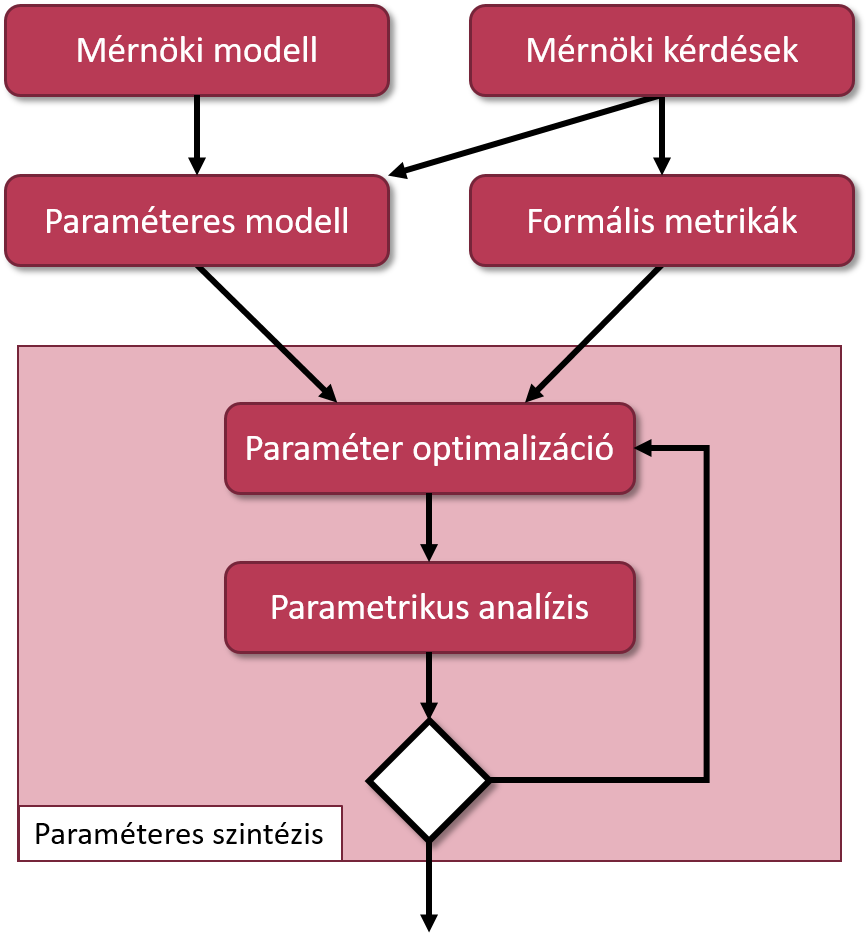
\includegraphics[width=90mm, keepaspectratio]{figures/abra.png}
	\caption{Paraméter optimalizálás folyamata.}
	\label{fig:folyamat}
\end{figure}

Egy modellben összefoglalhatjuk az összes jelentékeny tényezőjét a feladatnak. Kapcsolatokat definiálhatunk állapotok között, eseményeket köthetünk hozzájuk, úgy általában magunk előtt láthatjuk általa a rendszer viselkedését. Jó példa erre a Petri hálóval való modellezés. A Petri hálók tökéletesen alkalmasak információs folyamatrendszerek leírására és tanulmányozására, akár aszinkron, párhuzamos, nem-determinisztikus vagy sztochasztikus rendszerről van szó. Grafikus és matematikai eszköz is egyben, így lehetővé teszi számunkra, hogy matematikai viselkedéssel ruházzuk fel a rendszerünket, egyenlőségekkel, egyenletekkel, valószínűségekkel, paraméterekkel.\cite{PetriCikk}

Tulajdonképpen egy irányított gráfot definiálunk, melyben az irányított élek helyeket és átmeneteket kötnek össze. Minden helyen tetszőleges számban lehetnek "tokenek", melyek a folyamat nyomon követését teszik szemléletesebbé. Ha egy átmenetnél teljesülnek a tüzelési feltételek, az átmenet tüzel, és a bemenő helyeken lévő adott számú tokent a kimeneti helyek tokenjeivé "alakítja át".

A rendszer ilyen szintű megismerése után fontos mérföldköve a tervezésnek olyan kérdések keresése és feltevése, melyek kulcsfontosságúak lehetnek a rendszer működésében. Mikor következik be? Mik hatnak egymásra? Milyen kapcsolat van közöttük? Hogyan befolyásolja a folyamatot? A jó kérdések feltevése nem könnyű, de elengedhetetlen ahhoz, hogy újabb lépéseket tudjunk tenni a célunk felé.

A kérdések tulajdonképpen informális megfogalmazásai olyan matematikai összefüggéseknek, melyek a rendszerünk viselkedésében játszanak jelentős szerepet. Ezek a reward függvények olyan metrikákat írnak le, melyek kimenete mérhető. 

Ritka eset az, amikor teljes körű ismerettel rendelkezünk egy probléma minden részletéről. A legtöbb esetben elhanyagoljuk, vagy ismeretlen változóként a modellben hagyjuk azokat a részleteket, tulajdonságokat, értékeket, amelyekről nincs tudomásunk. 
Sztochasztikus modell esetén valószínűségi eloszlásokról, várható értékekről, tüzelési valószínűségekről, rátákról beszélünk. Példáinkban a tüzelési valószínűségek exponenciális eloszlást követnek. Az exponenciális eloszlás rátája, $\lambda$
függhet a modell paramétereitől. Ezáltal befolyásolják a hatótényezők a rendszert. Konkrét példákat a \ref{sec:meresek}. fejezetben mutatok be.

A metrikáink függenek ezektől a paraméterektől, azonban ennek a függésnek az alakját, tulajdonságait nem ismerjük. Ahhoz, hogy megtaláljuk egy sokdimenziós modell esetén azt az optimális paraméterlekötést, mellyel a rendszer teljesíti a követelményeket, paraméterszintézis során alkalmazunk különböző optimalizáló algoritmusokat.

A szintézis minden iterációjában újabb és újabb paraméterekkel futtatjuk le az analízist, majd az adott algoritmus működése alapján műveleteket végzünk a kapott eredményen, mely alapján eldönthetjük, elértük-e a leállási feltételt, és ha nem, az értelmezési tartomány mely pontjának a kiértékelése visz minket a legnagyobb valószínűséggel közelebb az optimális ponthoz. Ez lesz az a pont, amelyre a szintézis következő iterációjában megismételjük az elvégzett műveleteket.

A célfüggvény, melyet optimalizálunk, sokféleképpen definiálható. Mi az összes négyzetes hibát választottuk (\ref{eq:celfgv}), mely egy azon megközelítések közül, mellyel általánosan leírható egy rendszer elvárt viselkedéstől való eltérése.

\section{Algoritmusok használhatóságának szempontjai}

A paraméter optimalizálás során azt a pontot keressük, mely a rendszer hibáját 0-ra csökkenti. Ennek az elérését azonban számos tényező nehezíti, mind a tervező, mind az algoritmusok szempontjából.

Az analízist végző keretrendszer költségesen skálázódik a paraméterek dimenziójának növekedésével. Célunk egy olyan optimalizáló használata, mely ezt a költséget - mely a mi esetünkben főleg a futási időt jelenti - is minimalizálja.

Lehetőségünk van nemcsak függvényérték, de az egyes paraméterek szerinti érzékenység, vagyis parciális derivált kiszámítására is. Ennek köszönhetően szóba jöhetnek azok az ismert algoritmusok is, melyek egyszer, vagy többször differenciálható célfüggvényt feltételeznek. Tisztában kell lennünk azonban azzal, hogy ezért drága árat fizetünk, hisz a mi célfüggvényünk esetében (\ref{eq:celfgv}) egy gradiens számítás $O(n)$ számítást jelent, egy Hesse-mátrix $O(n^2)$ költséget jelentene, ahol a célfüggvény $j.$ paramétere szerinti parciális deriválja
$$\frac{\partial f}{\partial p_j}=\sum_{i=1}^{rewards}\left\lbrace   2\cdot \left( \hat{R}_i-R_i\right) \cdot\left(-\frac{\partial R_i}{\partial p_j}\right)  \right\rbrace   $$



Ahány ház, annyi szokás. Ahány programozó, annyi megvalósítás! Az algoritmusok hatékonyságában nagy szerepet játszanak a jól beállított hiperparaméterek. Ezek megtalálása közel olyan nehéz, mint maga a modell optimumának a megtalálása. Az algoritmusokat megkülönbözteti ez is, hogy mekkora teret engednek az algoritmus használójának, mennyi és milyen megkötésekkel, változókkal, feltételezett modellekkel egészíthető ki a modellünk a testreszabás érdekében. Minél jobban specializálható egy modellre az algoritmus, annál jobb eredményt érhetünk el az optimalizálás során.

Sztochasztikus, nemlineáris modelleket szeretnénk optimalizálni. Ezeknek az ismeretlen célfüggvényeinek megvan az a sajnálatos tulajdonsága, hogy bizonyos pontokban nem értelmezhetőek. Ezen pontok (területek), akár csak maga függvény alakja, természetesen nem ismertek. Fekete doboz kényszerek mellett keressük a fekete doboz függvényünk globális minimumát. % :D 
Elengedhetetlen tehát a hatékony működés érdekében, hogy -- jobb esetben -- elkerüljük az iterációk során ezen kiértékelhetetlen pontokat, vagy -- rosszabb esetben -- valamiképp kezelni tudjuk az algoritmus futása során ezen kiértékelhetetlen pontok számítására való igényt.

Összefoglalva tehát az alábbi szempontok alapján fogom vizsgálni a következő fejezetekben kipróbált optimalizáló algoritmusokat:

\begin{enumerate}
	\item Futási idő
	\item Deriváltak használatának szükségessége
	\item Hiperparaméterek mennyisége, minősége
	\item Kényszerek implementálhatósága
	\item Iterációk során kiszámítható és nem kiszámítható pontok aránya
\end{enumerate}











%----------------------------------------------------------------------------
\chapter{Algoritmusok}
\label{sec:algoritmusok}
%----------------------------------------------------------------------------

%----------------------------------------------------------------------------
\section{Nemkorlátos optimalizáló algoritmusok}
%----------------------------------------------------------------------------

\subsection{Newton módszer}
A Newton módszer\footnote{Newton's method} alkalmas nemkorlátos differenciálható függvények gyökeinek a megtalálására. Ezt felhasználva, $f(x)=0$ helyett $g(x)=f'(x)=0$ egyenlet megoldásait keresve az $f$ függvény lokális szélsőértékeit találhatjuk me. Az iteráció egyes lépéseiben ehhez az alábbi képletet kell alkalmagznunk:
$$x_{n+1}=x_n-\gamma[Hf(x_n)]^{-1}\nabla f(x_n),$$ 
ahol $\gamma<1$ egy általunk megadható lépéshossz, $H$ a Hesse-mátrix, $\nabla f(x)$ pedig a gradiens.

A konvergálás várható ideje és iterációszáma nagyban függ attól, hogy az iteráció kezdőpontja mennyire esik közel a keresett gyökhöz. Mivel ez egy általunk megadott paraméter, rejteget magában nehézséget. Jó esetben viszont nagyon gyorsan tud jó eredményt szolgáltatni.

Láthatjuk, hogy a mi esetünkben ez több kívánni valót is hagy maga után: szükséges hozzá a második derivált számítása minden iterációban, csak lokális szélsőérték keresést biztosít, és nincs lehetőségünk a korlátok kezelésére. Szerencsére azonban nem kell teljesen lemondanunk az algoritmusról, mivel több olyan megvalósítása is létezik, lehetővé teszi olyan függvények optimalizálást, ahol a Hesse-mátrix nem áll rendelkezésünkre. Ezeket az algoritmusokat kvázi-Newton módszerekként emlegetjük.

\subsubsection{BFGS}
A feltalálóiról elnevezett Broyden–Fletcher–Goldfarb–Shanno algoritmus egy a nagyon hatékony optimalizáló algoritmusok közül. A kvázi-Newton családba tartozó módszer a Hesse-mátrixot egy minden iterációban a gradiens alapján frissített, becsült mátrixszal helyettesíti. Ezzel számítási költséget spórolhatunk. A módosított algoritmus a következő lépéseket hajtja végre, míg nem konvergálunk a megoldáshoz:
\begin{enumerate}
	\item $B_kp_k=-\nabla f(x_k)$ egyenlet megoldásával kiszámoljuk $p_k$ értékét, ahol $B_k$ mátrix a Hesse-mátrix közelítése, kezdeti értéke $B_0=I$ egységmátrix.
	\item Tetszőleges egydimenziós optimalizálással megkereshető az $f(x_k+\alpha p_k)$ függvény minimuma,
	\item amivel ezután $x_{k+1}=x_k+s_k$, ahol $s_k=\alpha _kp_k$.
	\item A becsült $B_k$ mátrixot a következő egyenlet alapján frissítjük, a gradienseket felhasználva:
	$$y_k=\nabla f(x_{k+1})-\nabla f(x_k), \quad B_{k+1}=B_k+\frac{y_ky_k^T}{y_k^Ts_k}-\frac{B_ks_ks_k^TB_k}{s_k^TB_ks_k}.$$
\end{enumerate}

Eggyel tovább fejlesztett verziója, a Limitált memóriájú BFGS pedig azt is biztosítja, hogy az iterációk során az átlagosnál jóval kevesebb memóriát használunk.

Az eredeti Newton módszernél megfelelőbb a mi céljainkra, mivel csak gradiens számítást igényel. A kezdőpontot azonban itt is nekünk kell megadni, és ebben az esetben sincsen biztosítva a globális optimalizálás.

\subsection{Gradiens módszer}

A gradiens módszer\footnote{Gradient descent} egy másik ismert megoldás az optimalizálásra. Arra a megfigyelésre alapul, hogy ha egy pontban a gradiens irányával ellentétes irányba megfelelően kis lépést teszünk, biztos, hogy a jelenlegi pontnál alacsonyabb helyre kerülünk. Megfelelően folytatva ezt a szekvenciát feltehetően egy lokális minimumba érkezünk. Az iterációs lépés tehát a következő:
$$x_{n+1}=x_n-\gamma _n\nabla f(x_n),\quad \textnormal{ahol}\quad \gamma _n=\frac{(x_n-x_{n-1})^T[\nabla f(x_n)-\nabla f(x_{n-1})]}{\|\nabla f(x_n)-\nabla f(x_{n-1})\|^2}.$$
Tehát minden lépésben a lépés nagyságát is módosítjuk a gradiens és a mozgás függvényében. A lokális minimumba való konvergálás ilyen módon biztosítva van. 

Az általunk befolyásolható paraméter itt is a kezdőpont, máshonnan indítva az algoritmust más stacionárius pontot találhat meg.
\subsection{Részecske raj optimalizációk}
A részecske raj optimalizálás\footnote{Particle swarm optimization} során a keresési térben részecskéket veszünk fel. Ezek a részecskék egy egyszerű matematikai formula alapján járják be a teret, miközben a saját maguk és a globálisan ismert eddigi minimumhely ismeretében számolják ki minden iterációban, merre tegyék meg a következő lépést. Az i. részecske sebességének és pozíciójának kiszámításához használt képlet:
\begin{equation}
	\label{eq:pso}
	v_{i+1}=\omega v_{i}+\phi _pr_p(p_{i}-x_{i})+\phi_gr_g(g-x_{i}), \quad\textnormal{majd ezzel}\quad x_{i+1}=x_i+v_{i+1}
\end{equation}
ahol $r_p, r_g \sim U(0,1)$ véletlen számok, $\omega, \phi_p$ és $\phi_g$ pedig általunk választott hiperparaméterek. Ezeknek a megválasztása nagy körültekintést igényel, hisz jelentősen befolyásolják az algoritmus eredményességét.

Minden új pozíció kiszámításakor a részecske ellenőrzi, kisebb függvényértékű helyre érkezett-e, mint a lokálisan vagy globálisan ismert minimum, és ha igen, frissíti a megfelelő értékeket.

Az algoritmus futása során lényegében úgy mozognak a részecskék, hogy adott mértékben az ismert legalacsonyabb hely felé, adott mértékben pedig az általuk ismert legjobb hely felé próbálnak tartani, mindkét tényezőt egy véletlen számmal súlyozva. Sejthető, hogy ezzel semmilyen biztosítékot nem garantálhatunk a végeredményt illetően. Bár a gradiens számítását itt megspóroljuk, a sok részecskéhez tartozó függvényszámítások olyan nagyobb költséget okozhatnak, mint egy gradienst is használó, de kevesebb iteráció alatt konvergáló algoritmus. Kellő számú részecskével, kellő számú iteráció alatt viszont jó eredmény érhető el.

A tervező döntése a sebességek kiszámításában szereplő hiperparaméterek értéke, a részecskék és iterációk száma, illetve a tér azon részének a kiválasztása is, melyen a részecskéket elhelyezi. Ebből a térből a részecskék ki tudnak lépni, így a korlátok kezeléséhez plusz logika beépítése szükséges az algoritmusba.

\subsubsection{Méh algoritmus}

A természetben számtalan helyen visszaköszönnek a matematika szépségei. Rengeteg algoritmus mintázható az élőlények viselkedéséről vagy a természeti jelenségekről. Ezt teszi a méh algoritmus is. A részecske raj optimalizációk családjába tartozó módszer szintén nem használ deriváltszámítást, viszont a részecskék mozgása hierarchikusabb az alap algoritmus véletlenszerű mozgásánál. 

A méhek úgy keresik meg a lehető legtöbb virágot tartalmazó területeket, hogy először felderítőket küldenek véletlenszerű helyekre, majd visszaérkezésük után azok a méhek toborozzák magukhoz a legtöbb segítőt, akik a legjobb helyeket találták. 
Az első $b$ db, legjobb területet találó méhek a lebjobb méhek, azon belül az első $e$ db legjobbak az elit méhek. Értelem szerűen az elit méhek kapják a legtöbb segítőt maguk köré, a legjobbak, akik nem elitek, náluk kevesebbet. A többi toborzó marad véletlenszerű területek felderítőjének.

Minden iteráció során a segítő méhek egy $r$ sugarú körben véletlenszerűen helyezkednek el a toborzójuk által talált legjobb pont körül. Ezt a számot aztán iterációnként adott mértékben csökkenthetjük, így koncentrálva minél jobban az optimális helyekre. Ha egy részecske az eddigi minimumnál jobb pontot talál, ő veszi át a toborzó szerepét, és az utána következő iterációban már hozzá viszonyítva helyezkednek el a többiek.

Így a biztatónak ígérkező területek jóval több részecske által kerülnek felderítésre, ezzel növelve a lehető legjobb terület megtalálásának valószínűségét. Azok a méhek, akik nem kerültek a legjobbak közé, folytatják véletlenszerű felderítésüket, ezzel biztosítva azt is, hogy van esélyünk az eddig esetleg elkerült globálisan optimális helyet is megtalálni.

Általunk megadandó paraméter itt a felderítők száma, hogy az első hány legjobb méh a legjobb, és azon belül az első hány legjobb az elit, ők hány segítőt toboroznak magukhoz, az iterációk száma, a keresési terület határai, a keresési kör sugara, és az iterációnként való csökkentési mértéke.

\subsubsection{Gradiens módszerrel ötvözve}

Sok esetben a célunk eléréséért nem egy, hanem egyszerre több algoritmus által nyújtott lehetőségeket kell kihasználnunk. A részecske raj algoritmusok globális keresési tulajdonsága csábító, de hatékonysága csekély. Ellenben a gradiens módszer, bár biztosítja egy minimumhely megtalálását, ennek globális voltáról nincs információja.

Ideális megoldás lehet, ha a két ismert algoritmust ötvözzük. Ennek egy megvalósítása, ha minden iterációban a részecskék \aref({eq:pso}) képlet alapján kiszámolják az új pozíciójukat, majd az ezután ismert globális minimumhelyről indulva végzünk néhány lépést a gradiens módszerrel. Ezáltal biztosíthatjuk a keresési tér bejárását globális optimum után kutatva, és az ígéretesnek tűnő pozíciókból nem kell a véletlenre bíznunk magunkat, hogy mennyire tudjuk megközelíteni a tényleges szélsőértéket, a gradiens használatával biztosra mehetünk. Arany középút, mely a költséges műveletet, a derivált számítást csak ott végzi el, ahol a legnagyobb a valószínűsége az optimális hely megtalálásának.

\subsection{Szimulált lehűtés}

Szintén egy természetből vett példát utánozó algoritmus a szimulált lehűtés\footnote{Simulated annealing}. Köztudott, hogy egy anyag részecskéi annál jobban mozognak, minél magasabb az anyag hőmérséklete. A hőmérséklet csökkenésével ez a mozgás lassul, míg végül ki nem alakul a szilárd anyagra jellemző szabályos kristályszerkezet.

Az optimalizáló algoritmusban a rendszerünket egy kezdeti hőmérséklettől indítjuk, és ezt minden iterációban egy meghatározott arányban csökkentjük. A jelenlegi pozíciónk körül egy R sugarú körben kiválasztunk egy véletlenszerű pontot, majd eldöntjük, oda ugrunk e. Ez a döntés egy olyan valószínűséget adó egyenleten kell, hogy alapuljon, aminek az eredményéül magas hőmérséklet esetén nagy valószínűséggel a jelenleginél kedvezőtlenebb helyekre is átugrunk, a hőmérséklet csökkenésével azonban egyre kevésbé kockáztatunk. Ezzel csökkenthető annak az esélye, hogy egy lokális minimumba ragad a rendszer.
Valószínűséget adó egyenlet az én esetemben:

EGYENLET!! KÉT SOROS
% TODO

Ahol T a rendszerünk jelenlegi hőmérséklete. Amennyiben a visszatérési érték nagyobb egy $r\sim U(0,1)$ eloszlású véletlen számnál, végrehajtjuk az ugrást. Ellenkező esetben nem változtatunk a pozíciónkon. Annak az érdekében, hogy több lehetőséget adjunk az ugrásra, beiktatható egy ciklus, hogy 2-3 alkalommal próbálkozzon a rendszer ugyanazon hőmérsékletén új pozícióba jutni.

Egyszerűsége miatt közkedvelt algoritmus, hiszen itt sincs szükség derivált számítására. Hasonlóan azonban az előzőekhez, a hiperparaméterek beállítása itt is nagy hatással lehet az eredményességre.

Általunk megadandó paraméter a kezdeti hőmérséklet, a hőmérséklet iterációnként való csökkentésének aránya, a keresés R sugarának nagysága, és a csökkentésének az aránya.

%----------------------------------------------------------------------------
\section{Bayesi optimalizáció}
%----------------------------------------------------------------------------
A Bayesi optimalizáció módszere eltér az eddig megismert algoritmusokétól. Fix képletek helyett megpróbáljuk az iterációk során megtanulni a modellünk viselkedését, az eddigi kiértékelt pontok és a belőlük számított előzetes becslések alapján. Nagy számításigényű sztochasztikus rendszereink esetében ez egy ideális működés, mivel minimális kiértékelésre törekszünk azáltal, hogy a becslések alapján a legígéretesebbnek tűnő helyen számítjuk ki a függvényértéket.
\subsection{Gépi tanulás}
A gépi tanulás\footnote{Machine learning} a számítástudomány azon területe, mely képessé teszi a számítógépeket a tanulásra anélkül, hogy azt közvetlenül leprogramoznánk. Kapcsolódik a számítási statisztikákhoz, melyek célja előfeltételezések, jóslások számítása a rendszerhez, még a kiértékelése előtt. Többek között ezért a matematikai optimalizálásban is nagyon jó eszköznek bizonyult.

A kernel gépek a mintaelemzéses algoritmusok egy fajtája. Fő célja az adatok közötti kapcsolatok tulajdonságainak a vizsgálata és megismerése. Jellemzőjük, hogy tanulásuk során megjegyzik az összes eddigi bemenetüket és kimenetüket. Egy ismeretlen paraméterlekötés esetén annak kiértékelt értékét az ismert értékek és a kernel függvény segítségével becsülik meg.

\subsection{Gauss-folyamat}
A Gauss-folyamatok praktikus valószínűségi megközelítést nyújtanak a kernel gépekkel való tanuláshoz. 

Egy sztochasztikus folyamat valójában egy valószínűségi eloszlás -- mely leír egy véges dimenziójú véletlen valószínűségi változót -- általánosítása függvényekként. Azon folyamatokat, melyek esetében ez egy normális eloszlás, Gauss-folyamtoknak nevezzük.

Segítségükkel kétféle szempontból is tanulmányozhatjuk a modelljeinket. A regresszió lehetővé teszi a célfüggvényünk alakjának modellezését, ami által minden iteráció során előfeltételezéssel élhetünk az ismeretlen helyek függvényértékeiről is, és ezt felhasználva irányíthatjuk az optimalizáló algoritmust. Ez a feltételezett modell minden újabb megismert ponttal módosul, precízebb és -- reményeink szerint -- valósághűbb lesz.

A klasszifikáció diszkrét osztályokba sorolja a tér pontjait. A mi esetünkben egy bináris osztályozásról beszélhetünk azt tekintve, az értelmezési tartomány adott pontján a megoldó keretrendszer által kiértékelhető-e (1), vagy nem (-1) a modell. A regresszióhoz hasonlóan itt is minden iterációval frissítjük a becsült modellünket, melyet felhasználva feltételezéseket vonhatunk le, a tér egyes területein valószínűleg értelmezhető-e a célfüggvényünk.\cite{GPKonyv}


\subsection{Bayesi optimalizáció}
A Bayesi optimalizáció egy olyan, függvények fölötti a posteriori\footnote{Tapasztalatból származó ismeret} eloszlással dolgozik, mely a legjobban leírja a függvényt, melyet optimalizálunk. Ahogy a megfigyelt értékek száma nő, a jósolt eloszlásunk úgy válik biztosabbá. Amint egyre nagyobb valószínűséggel tudjuk megállapítani, mely területek a legérdemesebbek az újabb iterációkra, és ezáltal a modell pontosabbá tételére, úgy válik az algoritmus egyre hatékonyabbá.

Az algoritmus működése egyszerű és nagyszerű, az alábbi lépéseket ismétli, míg nem teljesül a megállási feltétel. Ez általában a végzendő iterációk számára vonatkozik.
\begin{enumerate}
	\item Tesztpontokkal való kezdeti modell betanítása.
	\item Nyereség függvény\footnote{Acquisition function} maximumának megkeresése a modell alapján.
	\item Célfüggvény kiértékelése a talált helyen.
	\item Modell frissítése a kiértékelt ponttal.
\end{enumerate}

\subsubsection{Nyereség függvény}
A Gauss folyamat által felállított modell várhatóérték függvénye nem áll rendelkezésünkre zárt alakban, így nem tudunk róla semmilyen konkrét információt sem. A nyereség függvény használatával ezt a problémát át tudjuk hidalni az algoritmus futása során. 

A nyereség függvény az értelmezési tartomány pontjaihoz egy olyan értéket rendel, mely kifejezi, mennyire lenne hasznos az adott ismeretlen pontot kiértékelni a modell javítása érdekében, az ismert pontok értékeinek függvényében. Ennek a függvénynek a maximumát keressük, és itt fogjuk a következő kiértékelést elvégezni, az eredménnyel pedig a modellt frissíteni.

A tervező döntése a megfelelő nyereség függvény kiválasztása. Hasznos lehet többet is kipróbálni, esetleg ötvözni őket, hisz érthető módon ez is befolyásolhatja az algoritmus hatékonyságát.

Leggyakoribb nyereség függvények\cite{AcqFgvCikk}:
\begin{itemize}
	\item Javulás valószínűsége\footnote{Probability of improvement}\\
	\begin{equation}
	\label{eq:POI}
		f_{PI}(x;\left\lbrace x_n,y_n\right\rbrace ,\theta)=\Phi(\gamma(x)), \qquad \gamma(x)=\frac{f(x_{best})-\mu(x;\left\lbrace x_n,y_n\right\rbrace ,\theta))}{\sigma(x; \left\lbrace x_n,y_n\right\rbrace ,\theta)},
	\end{equation}
	ahol $\left\lbrace x_n,y_n\right\rbrace$  kifejezés jelenti az eddig ismert pontokban a függvényértékeket, $\theta$ egy hiperparaméter mely a modellhez igazítandó, $\Phi$ a standard normális eloszlás függvénye, a  $\mu$ az aktuális modell váratóérték függvénye, $\sigma$ pedig a modell szórásfüggvénye.
	\item Javulás várható értéke\footnote{Expected improvement}
	\begin{equation}
	\label{eq:EI}
		f_{EI}(x;\left\lbrace x_n,y_n\right\rbrace ,\theta)=\sigma(x;\left\lbrace x_n,y_n\right\rbrace ,\theta)(\gamma(x)\Phi(\gamma(x))+\phi(\gamma(x)),
	\end{equation}
	ahol $\phi$ a standard normális eloszlás sűrűségfüggvénye (eloszlásfüggvény integrálja).
	\item Alsó biztos határ\footnote{Lower confidence bound}
	\begin{equation}
	\label{eq:LCB}
		f_{LCB}(x;\left\lbrace x_n,y_n\right\rbrace ,\theta)=\mu(x;\left\lbrace x_n,y_n\right\rbrace ,\theta)-\kappa \sigma(x;\left\lbrace x_n,y_n\right\rbrace ,\theta),
	\end{equation}
	ahol $\kappa$ hiperparaméter hivatott kifejezni a kizsákmányolás és felderítés módszere közötti egyensúlyozás mértékét, amiről bővebben a következő alfejezetben olvashatunk.
\end{itemize}
Ezek az ismert függvények esetében már a maximum megtalálása jóval egyszerűbb, mint az ismeretlen célfüggvényünk esetében. Agy alkalmas optimalizáló algoritmus -- akár a fentebb említettek közül -- jóval kisebb költséggel oldja meg, mint az eredeti problémát. Ebben rejlik tehát a Bayesi optimalizáció titka.

\subsubsection{Kizsákmányolás vagy felderítés}
A kizsákmányolás\footnote{exploitation} vagy felderítés\footnote{exploration} dilemmája ismert számos tudományterületen. Az optimalizálás során ugyanúgy hasznos az új tudás szerzése ismeretlen függvényterületekről, ahogy szükségünk lenne a már ismert tudás pontosságának, hatékonyságának növelésére is. Az algoritmus futása során nagy kérdés, mikor éri meg jobban egy olyan területről választani kiértékelendő pontot, ahonnan még nincsenek információink, és mikor válik nagyobb hasznunkra az eddig ismert, ígéretesnek tűnő területek precízebb feltérképezése, a globális minimum megközelítése érdekében.

Ez a döntés szerencsére a javulás valószínűsége (\ref{eq:POI}) és várható értéke (\ref{eq:EI}) nyereség függvényekben implicit kódolva van. Az alsó biztos határ (\ref{eq:LCB}) esetében azonban nekünk kell a $\kappa$ változóval döntést hozni a megfelelő arányról.

\subsubsection{Kernel függvény}
A kernel, vagy más néven kovariancia függvények szintén nagyban kihatnak a Bayesi optimalizáció eredményére. Mint fentebb említettem, a Gauss folyamat a priori eloszlások összessége függvények felett.
Egy 0 várható értékű modell esetén a kernel függvény teljes mértékben leírja a Gauss folyamat viselkedését.
Általános esetben azonban a folyamat a priorjainak simaságát, periodikusságát, izotrópiáját és állandóságát adja meg.

Sztochasztikus rendszereknél gyakran használt kernel függvények:
\begin{itemize}
	\item Exponenciális/Laplace: $exp(-\alpha\|x-y\|), \quad \alpha>0$.
	\item Négyzetes exponenciális: $exp(-\alpha\|x-y\|^2), \quad \alpha>0$.
	\item Gamma exponenciális: $exp(-\alpha\|x-y\|^\gamma), \quad \alpha>0, 0<\gamma\le1$.
	\item Matérn 1/2: $\sigma^2exp\left( -\frac{\|x-y\|}{\rho}\right)$. 
	\item Matérn 3/2: $\sigma^2\left( 1+\frac{\sqrt{3}d}{\rho}\right) exp\left(\frac{\sqrt{3}\|x-y\|}{\rho}\right)$.
	\item Matérn 5/2: $\sigma^2\left( 1+\frac{\sqrt{5}\|x-y\|}{\rho}\frac{5\|x-y\|^2}{3\rho^2}\right) exp\left(\frac{\sqrt{5}\|x-y\|}{\rho}\right)$.
\end{itemize}
A képletekben $\alpha$ az euklideszi távolság skálázó paramétere, $\gamma$ a gamma eloszlás alakját meghatározó paraméter, $\rho$ a kovariancia nemnegatív hiperparamétere.\\

Összességében láthatjuk, hogy a Bayesi optimalizáció törekszik a minimális számítási költségre, és számos ponton ad lehetőséget a tervezőnek a testre szabásra. Gradiens számítást sem igényel (habár léteznek már azzal kibővített megoldások a hatékonyság növelése érdekében). 
A korlátok algoritmusba kódolására is van lehetőség, amit a későbbiekben látni fogunk. 
A legnagyobb biztató jel azonban a klasszifikáció nyújtotta lehetőség a függvénytér azon területeinek a megbecsülésére, ahol a függvényérték a megoldó keretrendszer által kiszámítható.


% !TeX spellcheck = hu_HU
% !TeX encoding = UTF-8
% !TeX program = xelatex
%----------------------------------------------------------------------------
\chapter{Implementációk}
\label{sec:implementaciok}
%----------------------------------------------------------------------------

%----------------------------------------------------------------------------
% TODO ide is lesz majd jobb cím
\section{Önálló laboratórium algoritmusai}
%----------------------------------------------------------------------------

%----------------------------------------------------------------------------
\section{Bayesi optimalizáció}
%----------------------------------------------------------------------------
\subsection{Sklearn használatával}
\subsection{Tensorflow használatával}
\subsection{Shogun toolbox használatával}

%----------------------------------------------------------------------------
\chapter{Mérési eredmények}
\label{sec:meresek}
%----------------------------------------------------------------------------
Az algoritmusok működését a saját laptopomon, egy virtuális gépen teszteltem, VirtualBox segítségével. Adataik:
\begin{center}
	\begin{tabular}{ll}
		\hline
		\textbf{Gép} & \\
		\hline
		Operációs rendszer & Windows 10 Pro\\
		Processzor & Intel(R) Core(TM) i3-3217U CPU @ 1.80GHz\\
		Memória (RAM) mérete & 4 GB\\
		\hline
		\textbf{Virtuális gép} & \\
		\hline
		Név & StochOpt\\
		Operációs rendszer & Ubuntu (64-bit)\\
		Alapmemória & 2549 MB\\
		SATA port 0 & StochOpt.vdi (Normál, 10 GB)
	\end{tabular}
\end{center}

A Szakdolgozat nevű image-ben telepítve lett az összes futtatáshoz szükséges csomag és alkalmazás. Ezeket a következő utasításokkal értem el:
\begin{lstlisting}
molnar@molnar-VirtualBox:~$ sudo apt-get install python-pip

molnar@molnar-VirtualBox:~$ pip install bayesian-optimization
molnar@molnar-VirtualBox:~$ sudo apt-get install mono-complete

molnar@molnar-VirtualBox:~$ clone https://github.com/GPflow/GPflowOpt
molnar@molnar-VirtualBox:~$ sudo pip install . --process-dependency-links

molnar@molnar-VirtualBox:~$ sudo add-apt-repository ppa:shogun-toolbox/nightly
molnar@molnar-VirtualBox:~$ sudo apt-get install python-shogun

molnar@molnar-VirtualBox:~$ sudo apt-get install default-jdk junit maven
\end{lstlisting}

\section{Modellek}
A tesztelést az alábbi modellekkel végeztem, melyek részletei \aref{sec:fuggelek} függelékben találhatóak.\\
\begin{center}
	\begin{tabular}{lcc}
		\textbf{Modell} & \textbf{Paraméterek} & \textbf{Reward függvények} \\
		\hline
		simple-server.pnml & 2 & 2 \\
		vcl\_stochastic.pnml & 7 & 7 \\
		hybrid\_cloud.pnml & 10 & 4\\
		philosophers\_3.pnml & 3 & 3\\
		philosophers\_5.pnml & 5 & 5\\
		philosophers\_7.pnml & 7 & 7\\
		philosophers\_9.pnml & 9 & 9\\
	\end{tabular}	
\end{center}


A következőekben \aref{sec:optimalizacios-megkozelitesek}. fejezetben felállított szempontrendszer szerint értelmezem és értékelem a különböző algoritmusok működését a mérések eredménye alapján.

%----------------------------------------------------------------------------
\section{Futási idő}
%----------------------------------------------------------------------------
A tesztesetek futási idejéről csak óvatosan tudunk következtetéseket levonni. Az eredmények alapján nemcsak a modellek nagysága, de főként a bonyolultsága is nagyban befolyásolja az egyes algoritmusok futási idejét, melyről így nem állapítható meg lineáris kapcsolat. Szintén, nem meglepő módon, nagy befolyásoló tényező az is, hogy az algoritmusok milyen pontokban kérdezik le a modell értékét, a megoldó keretrendszer válaszideje nagy változékonyságot mutat, a másodperc töredékétől ritka esetben akár 20 percig is terjedhet. A mérések átlagos alakulását \aref{fig:exectime}. ábra szemlélteti.
\begin{figure}[!ht]
	\centering
	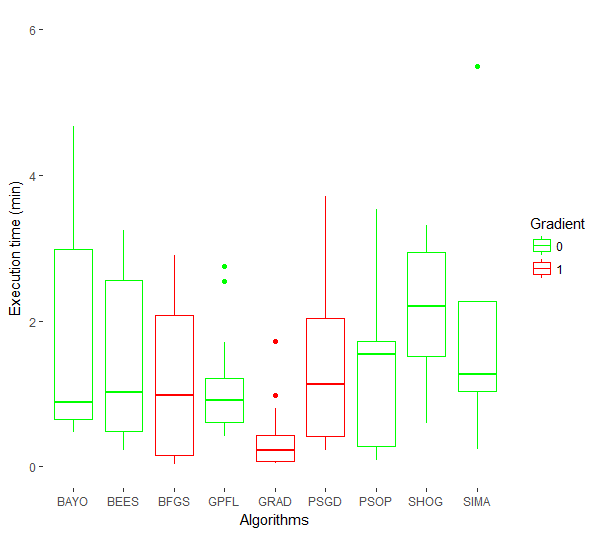
\includegraphics[width=140mm, keepaspectratio]{figures/execution_times_dobozdiagram.png}
	\caption{Algoritmusok átlagos futási ideje}
	\label{fig:exectime}
\end{figure}

Feltűnő a gradiens metódus átlagos futási idejének alacsony értéke, ez azonban csak annak tudható be, hogy az algoritmus, ha nem értelmezhető pontban szeretné kiszámolni az értéket, újraindul egy másik véletlen kezdőpontról, addig, míg el nem fogy a próbálkozásaink adott száma. Ennek a következményét \aref{fig:derivaltak}. ábrán láthatjuk is.

Jelenleg a leglassabbnak a Shogun toolbox-szal való Bayesi optimalizálás, illetve a részecske raj és a szimulált lehűtés tűnik. Nem kell azonban elkeserednünk, a további szempontok alapján tisztább képet alkothatunk az algoritmusokról.
%----------------------------------------------------------------------------
\section{Deriváltak használata}
\label{sec:derivaltak}
%----------------------------------------------------------------------------
Gradiens számítást az L-BFGS, a gradiens módszer és a részecske raj optimalizáció gradiens módszerrel való ötvözése igényel. Kérdés azonban, hogy mennyire jobb ezek hatékonysága a többi algoritmushoz képest?

Az mérési eredmények pontosságát \aref{fig:derivaltak}. dobozdiagrammon láthatjuk, összehasonlítva a deriváltakat használó és nem használó algoritmusokat. Az y tengely jelenti a mérés végeredményeként kapott pontban a célfüggvényünk értékét, a négyzetes hibaarányt. Azok tehát a leghatékonyabbak, melyek a legközelebb helyezkednek el a nullához.

A gradiens módszer hamar kiesett a sorból, hisz nem tud mit kezdeni a nem értelmezhető pontokkal. A szimulált lehűtés véletlen pontokba való ugrálása a bonyolult, nagy dimenziószámú modelleknél nem bizonyul hatékonynak. Úgy tűnik, a mi sztochasztikus eseteinkben még a közkedvelt L-BFGS algoritmus is elvesztette a versenyt, hiába rendelkezik a gradiens számítás látszólagos előnyével. A gradiens számítás lényege valójában csak a részecske raj optimalizációnál nyilvánul meg egyértelműen: a gradienst ismerő raj algoritmus átlagosan az optimumhoz közelebbi értékeket talált, mint az egyszerű függvényszámítást végző társai.

A többi algoritmus eredménye közül pedig jól látható, hogy a Bayesi algoritmusok tudták a nullához legközelebbi eredményeket produkálni.


\begin{figure}
	\centering
	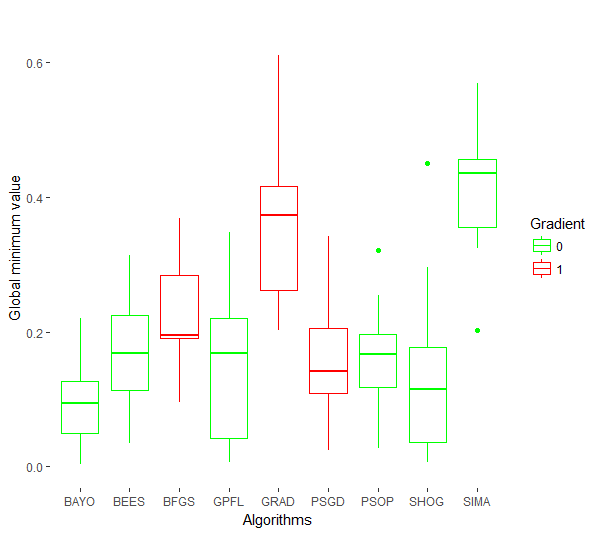
\includegraphics[width=140mm, keepaspectratio]{figures/gradiens_pontossag_boxplot.png}
	\caption{Optializáció átlagos pontossága algoritmusonként}
	\label{fig:derivaltak}
\end{figure}

Az algoritmusok átlagos számítási igénye \aref{fig:funccalc}. dobozdiagrammon látszik. Az y tengely értéke jelzi, hányszor hívták meg átlagosan a megoldó keretrendszer kiértékelését egy adott paraméter lekötéssel az algoritmusok.

Itt már gyönyörűen látszik a Bayesi optimalizációk elsöprő sikere. Az ő eseteikben csak azok a hívások történnek, melyek a kezdeti feltérképező pontok, majd iterációnként egy újabb pont kiszámítását jelentik, mellyel a regressziós ill. klasszifikációs közelítő modellünket frissítjük. Ellentétben a nemkorlátos algoritmusokkal, melyek vagy rengeteg részecskét igényelnek a terület kellően alapos bejárására, vagy rengeteg iterációt az eredmény konvergálásához. Mint fentebb már volt róla szó, a gradiens módszer látszólagos hatékonyságát itt is az okozza, hogy nagyon hamar feladja a próbálkozást nem értelmezhető pontba való érkezéskor.

\begin{figure}
	\centering
	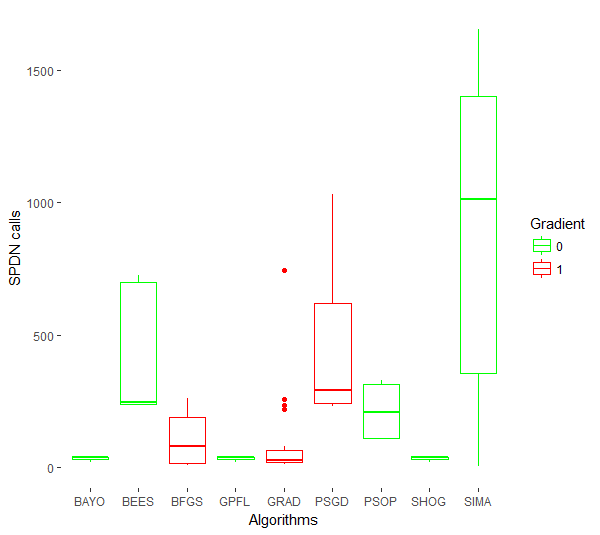
\includegraphics[width=140mm, keepaspectratio]{figures/func_calcs_boxplot.png}
	\caption{Megoldó keretrendszer hívásának száma algoritmusonként}
	\label{fig:funccalc}
\end{figure}

%----------------------------------------------------------------------------
\section{Hiperparaméterek}
%----------------------------------------------------------------------------
A mérésekben a legnagyobb nehézséget a sokféle algoritmus sokféle hiperparaméterének a beállítása jelentette. A változtatásuknak az eredménye helyenként megfeleltek a várakozásainknak, néhol azonban meglepő dolgokat tapasztalhatunk. Lássuk tehát a tanulságokat, mely paraméterek tűnnek dominánsnak az egyes algoritmusok esetében.
\paragraph{L-BFGS} \subparagraph{initPoint, restart} A hatékonyság leginkább azon múlik, megfelelő helyről indítjuk-e az algoritmust. Erről a ``megfelelő'' helyről azonban általában nincs tudomásunk, így minél többször indítjuk újra a futást, annál közelebb kerülhetünk az optimumhoz. Ezzel arányosan természetesen a futásidő is nő.
\paragraph{Gradiens módszer}\subparagraph{restart} Hasonló módon az L-BFGS-hez, a legnagyobb hasznot itt is a minél több próbálkozás hozza. Szerencsés esetben nagyon gyorsan tud az optimumba konvergálni, a mi nagy modelljeink esetében azonban az ilyen kezdőpont megtalálásának az esélye kicsi.
\paragraph{Részecske raj}\subparagraph{swarmSize, maxIter, fiParticle, fiGlobal} Modellenként más és más képet mutatnak az eredmények, nem állapítható meg domináns hiperparaméter. Volt példa a raj számának, vagy az iterációk számának a növelésével némi javulásra, helyenként azonban a fi-k értékének a megváltoztatása két nagyságrendű javulást is eredményezett. Ebből is látszik, hogy az optimalizáló algoritmusok nagy problémája, hogy a megfelelő hiperparaméter beállítás minden modellre specifikus.
\paragraph{Részecske raj, gradiens módszerrel}\subparagraph{swarmSize, maxIter, fiParticle, fiGlobal, gradientMaxIter} Az alap algoritmushoz képest a gradiens módszer iterációszámának a növelése az elvárásoktól eltérően nem javítja jelentősen az eredményt. Úgy tűnik néhány lépéssel elég jól megközelíthető a lokális optimum, újabb iterációkkal nem számottevő a javulás. 
\paragraph{Méh algoritmus}\subparagraph{maxIter} Számos hiperparaméterrel rendelkező algoritmus, melyekre itt is fennáll, hogy modellenként változó hatékonyságot mutattak az ugyanolyan beállításaik. A kiemelkedő azonban ebben az esetben az iterációk száma volt. A növelésével jelentősebb javulások voltak elérhetőek, mint a többi paraméter állításával. Az algoritmus szépsége a felderítő és kizsákmányoló technika vegyítése, így nem meglepő, hogy minél tovább folytatjuk az algoritmus lépéseit, annál inkább feltérképezhető a függvénytér. Értelemszerűen ezért azonban nagy árat fizetünk, ahogy \aref{fig:funccalc}. ábrán is láthattuk.
\paragraph{Szimulált lehűtés}\subparagraph{$\emptyset$} Az  ábrázolt dobozdiagrammokon már láthattuk, hogy ez az algoritmus nem felel meg hatékonyságban az elvárásainknak. A mérési eredmények külön vizsgálásakor sem derül ki újabb információ. Hiperparaméter lehetőségei nem elég kifinomultak a mi modelljeink megfelelő mértékű optimalizálásához.
\paragraph{Bayesi optimalizálás, Scikit-learn csomaggal}\subparagraph{acq\_param, n\_iter, init\_points} Izgalmas dolgot tapasztalhatunk a nyereség függvény paraméterének a beállításakor. Ez a paraméter minél nagyobb, annál inkább tolódik az algoritmus a felderítő, és nem a kizsákmányoló módszer felé. A mi eseteinkben a felderítő technika hoz szembetűnő javulást, ami a kisebb modelleknél főként a futásidő drasztikus csökkenésében mutatkozik meg, a nagyobb modellek esetében azonban az optimumot is sokkal jobban megközelítik az ilyen beállítású mérések. Ezen kívül itt az iterációk és kezdőpontok száma közül az iterációk növelésével finomítható nagyobb mértékben a végeredmény.
\paragraph{Bayesi optimalizálás, TensorFlow-val}\subparagraph{init\_points} Bár kipróbáltam a jót sejtető kernel és nyereség függvény opciókat, semmilyen változást nem produkáltak. Több tizedesjegy nagyságban ugyanazokat a pontokat találták meg az algoritmus variánsok, csupán a futásidők különböztek, de azok sem szabályosan, valószínűsíthető, hogy ezt csak a keretrendszer válaszideje produkálta. Ami azonban kiderült, hogy ennél az implementációnál a kezdőpontok számán van a hangsúly! Minél több kezdeti ponttal állítjuk fel a becsült modellünket, annál precízebb eredményt kapunk, viszonylag kevés iterációszámmal is.
\paragraph{Bayesi optimalizálás, Shogun-toolbox-szal}\subparagraph{init\_points} Saját implementációjú Bayesi optimalizációmnak viszonylag kevés hiperparamétere van: a kezdőpontok és iterációk száma. A mérések során kiderült, hogy ebben az esetben is a kezdőpontok száma bír nagyobb befolyással a végeredményre, sokkal jobb hibaérték érhető el, és nem utolsó sorban a futási idő is barátságosabb, mint ha az iterációk számát növelnénk helyette.

%----------------------------------------------------------------------------
\section{Kényszerek implementálhatósága}
%----------------------------------------------------------------------------
A paraméterekre vonatkozó ismert korlátok kezelhetősége látványos különbséget mutat a nem korlátos és a Bayesi algoritmusok között. Ezek azok a korlátok, melyet a modellt ismerő szakértő tud megmondani a paraméterek értelmezési tartományáról. Hiszen egyértelmű, hogy egy időt jelölő paraméter nem vehet fel negatív értéket, vagy egy valószínűségi érték 1-nél nagyobb számot.

A nem ismert korlátok\footnote{black-box constraints} -- vagyis a függvénytér nem értelmezhető területeinek -- kezelésére a nemkorlátos algoritmusok esetén nem volt jó megoldásunk. Az L-BFGS, gradiens módszer és szimulált lehűtés esetén egyszerűen félbehagytuk az optimalizálást, és megpróbáltuk újrafuttatni az elejétől, másik kezdőpontból. A részecske raj algoritmusoknál ilyen esetben pedig csak egy konstans nagy értéket adtunk függvényértékül a részecskének, ezzel elkerülve a hosszas véletlenszerű próbálkozásokat minden részecske esetén, aki ilyen területre téved.

A mérési eredményekről egy átlagos képet mutatni ebben az esetben nem lenne praktikus, mivel az elvárt értékektől való eltérés egyes esetekben 20-30 nagyságrendnyi. Ehelyett  \aref{table:globalminimumpoints}. táblázat egy-egy konkrét futási eredményt tartalmaz, melyből nagyságrendileg láthatjuk, az algoritmusok mennyire képesek megközelíteni az általunk elvárt globális minimumpontot, a különböző bonyolultságú modellek esetében. Pirossal kijelölve láthatóak azok a pontok, melyek az elvárttól nem tértek el több nagyságrendnyire.

A talált, és az általunk várt minimumpont különbsége jól mutatja a Bayesi optimalizálás nagyszerűségét a többi, véletlenekre és gradiensekre alapuló algoritmussal szemben. A nemkorlátos algoritmusok csak a legegyszerűbb modellünknél tudták felvenni a versenyt, ott azonban mérhetően jobban teljesítettek a Bayesi algoritmusoknál. A kétféle optimalizálási típus két különböző problémakörre lett kifejlesztve, és úgy tűnik, e két halmaz között nagyon kicsi az átfedés.

\begin{table}
	\fontfamily{pcr}\selectfont
	\fontsize{8}{9.5}\selectfont
	\center
	\begin{tabular}{ll}
		\hline
		\textbf{phil\_3} &\textit{(7.33 2.15 9.68)}\\
		\hline
		BFGS & (1.14E24 2.54E7 1.08E19)\\
		GRAD & (8.73E24 2.39E8 2.79E33)\\
		PSOP & (1.08E15 120.01 3.28E15)\\
		PSGD & (9.55E22 10.12 1.02E39)\\
		BEES & (1.59 4.94E3 29.9)\\
		SIMA & (2.12E24 4.46E4 7.87E31)\\
		{\color{red}BAYO} & {\color{red}(7.34 3.19 77.71)}\\
		{\color{red}GPFL} & {\color{red}(54.6 2.4 80.1)}\\
		{\color{red}SHOG} & {\color{red}(25.67 2.28 14.54)}\\
		\hline
		\textbf{phil\_5} & \textit{(7.33 2.15 9.68 9.64 9.47)}\\
		\hline
		BFGS & (2.14E20 3.08E3 7.74E16 8.12E13 2.09E16)\\
		GRAD & (8.66E16 23.32 4.66E15 1.96E31 1.07E33)\\
		PSOP & (1.4E12 8.77E4 2.53E12 1.24E14 2.83E23)\\
		PSGD & (1.35E12 14.59E4 4.13E12 2.01E21 1.17E23)\\
		BEES & (3.58E18 1.18E6 4.59E17 1.66E17 4.04E14)\\
		SIMA & (3.44E29 7.63E2 3.21E10 1.44E24 2.63E27)\\
		{\color{red}BAYO} & {\color{red}(4.03 13.72 82.99 15.61 14.78)}\\
		{\color{red}GPFL} & {\color{red}(3.08 13.17 7.04 7.04 46.98)}\\
		{\color{red}SHOG} & {\color{red}(69.99 0.96 55.33 18.74 29.34)}\\
		\hline
		\textbf{phil\_7} & \textit{(7.33 2.15 9.68 9.64 9.47 4.03 3.01)}\\
		\hline
		BFGS & (2.43E15 5.51E7 7.23E14 1.57E9 6.04E10 2.82E15 7.51E9)\\
		GRAD & --\\
		PSOP & (8.25E16 8.96E2 3.97E31 3.13E26 1.23E37 3.75E7 5.95E6)\\
		PSGD & --\\
		BEES & (6.79E19 1.88E6 3.53E22 2.04E27 5.88E20 4.05E14 4.42E9)\\
		SIMA & (2.89E9 9.45E4 2.11E19 2.74E25 3.75E37 1.21E10 7.69E4)\\
		{\color{red}BAYO} & {\color{red}(69.29 1.56 88.98 84.87 3.31 5.66 6.27)}\\
		{\color{red}GPFL} & {\color{red}(12.50 7.08 45.45 45.45 2.74 15.87)}\\
		{\color{red}SHOG} & {\color{red}(22.64 1.83 84.58 11.99 9.34 24.52 3.01)}\\
		\hline
		\textbf{phil\_9} & \textit{(7.33 2.15 9.68 9.64 9.47 4.03 3.01 1.24 6.63)}\\
		\hline
		BFGS & (1.93E22 14.03 1.07E39 6.67E32 7.52E8 1.46E17 1.5E4 2.67E3 1.84E14)\\
		GRAD & (1.75E12 5.889E5 7.73E37 1.22E26 1.39E22 2.54E11 5.51E9 14.87 1.77E24)\\
		PSOP & (1.69E23 29.23E2 1.99E21 1.17E11 4.38E10 1.64E7 8.93E7 126.0 3.51E21)\\
		PSGD & (1.42E9 7.58E4 2.8E19 1.67E29 9.38E22 1.39E15 9.42E9 5.43E2 6.73E18)\\
		BEES & (1.62E7 2.55 6.51E33 6.3E22 4.53E22 1.2E4 8.36E7 3.15 4.31E22)\\
		SIMA & (2.79 1.26E8 7.79E37 2.78E4 2.62E29 34.9 7.74E12 3.93E4 3.08E17)\\
		{\color{red}BAYO} & {\color{red}(0.80 9.95 89.34 5.61 80.63 7.78 1.9 1.11 59.96)}\\
		{\color{red}GPFL} & {\color{red}(5.47 1.56 7.04 7.04 10.11 37.26 7.46 2.14 31.32)}\\
		{\color{red}SHOG} & {\color{red}(40.59 7.54 129.4 137.5 18.91 9.02 0.85 5.5 16.55)}\\
		\hline
		\textbf{smpl} & \textit{(1.5 0.25)}\\
		\hline
		{\color{red}BFGS} & {\color{red}(1.5 0.25)}\\
		{\color{red}GRAD} & {\color{red}(1.5 0.25)}\\
		{\color{red}PSOP} & {\color{red}(14.08 0.87)}\\
		{\color{red}PSGD} & {\color{red}(1.5 0.25)}\\
		{\color{red}BEES} & {\color{red}(1.49 0.25)}\\
		SIMA & (1.49E3 7.48)\\
		{\color{red}BAYO} & {\color{red}(2.64 0.74)}\\
		{\color{red}GPFL} & {\color{red}(3.27 0.54)}\\
		{\color{red}SHOG} & {\color{red}(1.81 0.68)}\\
		\hline
		\textbf{vcls} & \textit{(0.015 0.5 0.15 60 . 0.75 0.6)}\\
		\hline
		BFGS & --\\
		GRAD & --\\
		PSOP & --\\
		PSGD & --\\
		BEES & --\\
		SIMA & --\\
		{\color{red}BAYO} & {\color{red}(0.02 38.21 10.63 304.3 499.8 0.56 0.66)}\\
		{\color{red}GPFL} & {\color{red}(0.78 26.31 7.1 3.47E3 289.5 0.0075 0.006)}\\
		{\color{red}SHOG} & {\color{red}(1.31 21.32 11.92 594.8 41.86 3.89 0.58)}\\
		\hline
		\textbf{hybc} & \textit{(5 0.75 0.0002 0.2 0.1 0.0002 0.1 24 0.8 0.3 0.01 1000)}\\
		\hline
		BFGS & --\\
		GRAD & --\\
		PSOP & (12.21 1.48 1.002 1.27 2.17 1.001 1.019 1.52E11 2.33 1.68 1.02 1.67E-66)\\
		PSGD & --\\
		BEES & --\\
		SIMA & --\\
		{\color{red}BAYO} & {\color{red}(3.69 0.37 0.0008 0.11 0.71 0.0004 0.05 27.75 0.67 0.06 0.009 139.9)}\\
		{\color{red}GPFL} & {\color{red}(2.42 0.99 0.0005 0.26 0.21 0.0005 0.02 22.1 0.38 0.18 0.06 2084.2)}\\
		{\color{red}SHOG} & {\color{red}(2.8 0.22 0.002 0.07 0.97 0.0003 0.09 29.81 0.88 0.97 0.002 1362.7)}\\	
	\end{tabular}
	\caption{Talált globális minimumpontok modellenként és algoritmusonként}
	\label{table:globalminimumpoints}
	\begin{tablenotes}
		A bonyolultabb modellekkel sok algoritmus nem tudott megbírkózni, futásuk alatt nem találtak kiszámítható pontot. Ezeket -- jellel jelöltem a táblázatban
	\end{tablenotes}
\end{table}
%----------------------------------------------------------------------------
\section{Értelmezhető - nem értelmezhető területek aránya}
\label{sec:teruletek}
%----------------------------------------------------------------------------
Mivel fő célunk a sztochasztikus modellek optimalizálása, nem ismert korlátokkal, az algoritmusok hatékonyságát nagyban jellemzi, hogy a kiszámított pontok közül hány értelmezhető, és hány nem. Egy olyan algoritmust keresünk, ami megtalálja a kiszámítható területeket, és ott végez kimerítő keresést, ezáltal kevés számítást pazarolva a nem értelmezhető területekre.

A modellek közül a philosophers\_9.pnml egy azok közül, melyek optimalizálása során nagy számban futottak nem értelmezhető területekre az algoritmusok. Az átlagos eloszlását ezen területeknek \aref{fig:ertelmezhetopontok}. ábrán láthatjuk.

\begin{figure}[!ht]
	\centering
	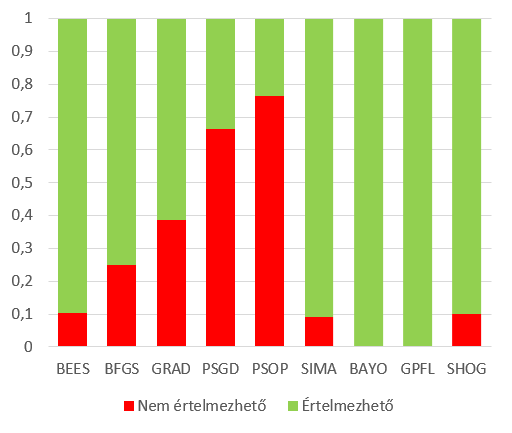
\includegraphics{figures/fil9pontaranyok.png}
	\caption{Számítható és nem számítható pontok eloszlása az algoritmusokat a philosophers\_9 modellen futtatva}
	\label{fig:ertelmezhetopontok}
\end{figure}

A Bayesi algoritmusok esetében a Gauss folyamat modelljét alakítani tudjuk az eddigi információink alapján. Erre két példát mutattak az implementációim: nem értelmezett pont értékén egy konstans nagy büntetőérték adása, mellyel biztatni szeretnénk a regressziós modellt arra, hogy itt ne keressen tovább minimumom, illetve a klasszifikáció eszközével, amikor egyértelműen tároljuk a kiszámított pontokról, értelmezhetőek-e, vagy sem, és ennek a valószínűsége is szerepet játszik a nyereség függvényben. Ennek az eredményessége egyértelműen látszik a halmozott oszlopdiagrammon, bár sajnálatos, hogy a klasszifikáció megvalósítása a \texttt{MyShogunOpt} osztályban még nem olyan hatékony, mint a \texttt{GPFlowOpt} és a \texttt{BayesianOptimization} Python implementációk esetében a büntető érték használata.


\chapter{Összefoglalás}


% Acknowledgements
%~~~~~~~~~~~~~~~~~~~~~~~~~~~~~~~~~~~~~~~~~~~~~~~~~~~~~~~~~~~~~~~~~~~~~~~~~~~~~~~~~~~~~~
%----------------------------------------------------------------------------
\chapter*{\koszonetnyilvanitas}\addcontentsline{toc}{chapter}{\koszonetnyilvanitas}
%----------------------------------------------------------------------------



% List of Figures, Tables
%~~~~~~~~~~~~~~~~~~~~~~~~~~~~~~~~~~~~~~~~~~~~~~~~~~~~~~~~~~~~~~~~~~~~~~~~~~~~~~~~~~~~~~
%\listoffigures\addcontentsline{toc}{chapter}{\listfigurename}
%\listoftables\addcontentsline{toc}{chapter}{\listtablename}


% Bibliography
%~~~~~~~~~~~~~~~~~~~~~~~~~~~~~~~~~~~~~~~~~~~~~~~~~~~~~~~~~~~~~~~~~~~~~~~~~~~~~~~~~~~~~~
%\bibliography{bib/mybib}
%\addcontentsline{toc}{chapter}{\bibname}
% TODO megcsinálom majd szépre!

\begin{thebibliography}{widestlabel}
	\bibitem{MarkovLancokKonyv} Györfi László és Páli István, Tömegkiszolgálás informatikai rendszerekben, Műegyetemi Kiadó 2001
	\bibitem{SolverKonyv} Yousef Saad, Iterative Methods for Sparse Linear Systems, 2000
	\bibitem{ParameterSzintezisCikk} Tim Quatmann, Christian Dehnert, Nils Jansen,	Sebastian Junges, and Joost-Pieter Katoen, Parameter Synthesis for Markov Models: Faster Than Ever, RWTH Aachen University, University of Texas at Austin, 2016, \url{https://arxiv.org/pdf/1602.05113.pdf}
	\bibitem{SpdnTDK} Marussy Kristóf és Kleinik Attila, Aszinkron rendszerek konfigurálható sztochasztikus analízisét támogató keretrendszer, 2015
\end{thebibliography}


% Appendix
%~~~~~~~~~~~~~~~~~~~~~~~~~~~~~~~~~~~~~~~~~~~~~~~~~~~~~~~~~~~~~~~~~~~~~~~~~~~~~~~~~~~~~~
% %----------------------------------------------------------------------------
\appendix
%----------------------------------------------------------------------------
\chapter*{\fuggelek}\addcontentsline{toc}{chapter}{\fuggelek}
\setcounter{chapter}{\appendixnumber}
%\setcounter{equation}{0} % a fofejezet-szamlalo az angol ABC 6. betuje (F) lesz
\numberwithin{equation}{section}
\numberwithin{figure}{section}
\numberwithin{lstlisting}{section}
%\numberwithin{tabular}{section}

%----------------------------------------------------------------------------
\section{Modellek}
\label{sec:fuggelek}
%----------------------------------------------------------------------------
\subsection{Simple server}

Egy számítógépes szerver modellje, végtelenül leegyszerűsítve. Paramétereink a felhasználói kérések érkezésének rátája, illetve azok kiszolgálásához szükséges idő. Reward függvényeink azt mondják meg, mennyi időt töltünk várakozó állapotban, és hogy milyen gyakorisági rátával tudjuk kiszolgálni az egyes kéréseket.
\begin{center}
	\begin{tabular}{cc}
		\textbf{\textbf{Paraméter}} & \textbf{Default érték} \\
		\hline
		requestRate & 1.5\\
		serviceTime & 0.25\\
	\end{tabular}
	\label{table:filparam}
	\quad
	\begin{tabular}{c}
		\textbf{\textbf{Reward függvény}}\\
		\hline
		Idle\\
		ServedRequests\\
	\end{tabular}
	\label{table:filrewards}
\end{center}
\begin{figure}[!ht]
	\centering
	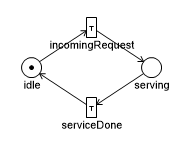
\includegraphics{figures/smpl.png}
	\caption{Egyszerű szerver modellje a PetriDotNet alkalmazásban}
\end{figure}

\subsection{VCL stochastic}

TODO miez?
\begin{center}
	\begin{tabular}{lrl}
		\textbf{\textbf{Paraméter}} & \textbf{Default érték} & \textbf{Leírás} \\
		\hline
		incomingRate & 0.015 & Beérkező kérések rátája\\
		dispatchTime & 0.5 & Kérés dispatch ideje\\
		warmDispatchTime & 0.15 & További dispatch idő meleg gép esetén\\
		jobTime & 60 & Feladatok végrehajtásának átlagos ideje\\
		powerTime & 5 & Gép ki- vagy bekapcsolásának ideje\\
		powerUsage & 0.75 & Gép energiaigénye időegységenként\\
		idlePowerFactor & 0.6 & Várakozó gép energiaigénye\\
	\end{tabular}
	\quad
	\begin{tabular}{ll}
		\textbf{\textbf{Reward függvény}} & \textbf{Leírás}\\
		\hline
		jobsFinished & Befejezett feladatok\\
		powerUsage & Energia felhasználás\\
		noFreeMachines & Szabad gépek hiánya\\
		jobsDispatched & ??\\
		machinesWorking & Működő gépek\\
		hotMachinesWorking & Működő meleg gépek\\
		coldStarted & Elindított hideg gépek\\
	\end{tabular}
\end{center}

\begin{figure}
	\centering
	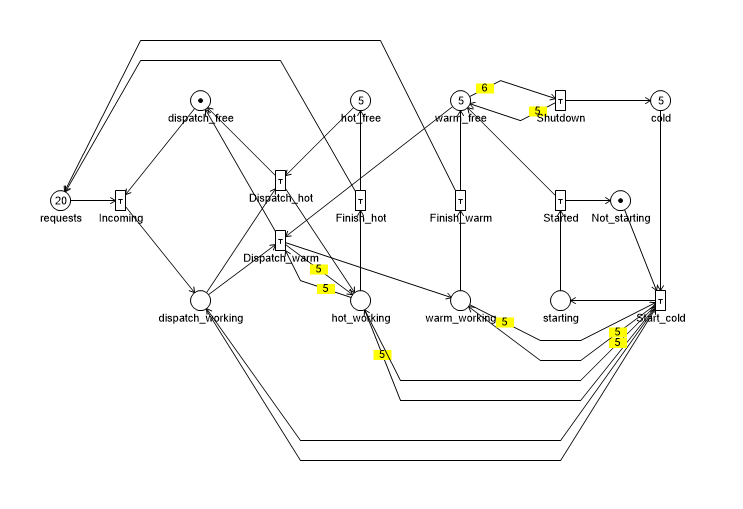
\includegraphics[width=140mm, keepaspectratio]{figures/vcl.png}
	\caption{Sztochasztikus VCL ?? modell a PetriDotNet alkalmazásban}
\end{figure}

\subsection{Hybrid cloud}

Egy sztochasztikus felhő alkalmazás modellje.
\begin{center}
	\begin{tabular}{lrl}
		\textbf{\textbf{Paraméter}} & \textbf{Default érték} & \textbf{Leírás} \\
		\hline
		incRate & 5& Beérkező kérések rátája\\
		p & 0.75 & Privát felhő dispatch valószínűsége\\
		lbTime & 0.0002 & Load balancer elindítához szükséges idő\\
		execTime1 & 0.2 & Publikus felhő végrehajtási ideje\\
		execTime2 & 0.1 & Privát felhő végrehajtási ideje\\
		failRate & 0.0002 & Privát szerverek hibarátája\\
		idleFactor & 0.1 & Várakozó gépek relatív igénybevétele\\
		repairTime & 24 & Privát szerverek javítási ideje\\
		publicRent & 0.8 & Óránkénti foglalás publikus felhőn\\
		runPower & 0.3 & Egy működő gép üzemeltetési költsége\\
		idlePower & 0.01 & Egy várakozó gép üzemeltetési költsége\\
		repairCost & 1000 & Gép javításának költsége\\
	\end{tabular}
	\quad
	\begin{tabular}{ll}
		\textbf{\textbf{Reward függvény}} & \textbf{Leírás}\\
		\hline
		Expense & Költség\\
		JobComplete & Teljesített feladatok\\
		JobsProcessing & Folyamatban lévő feladatok\\
		NoFailedServer & Működő szerverek\\
	\end{tabular}
\end{center}

\begin{figure}
	\centering
	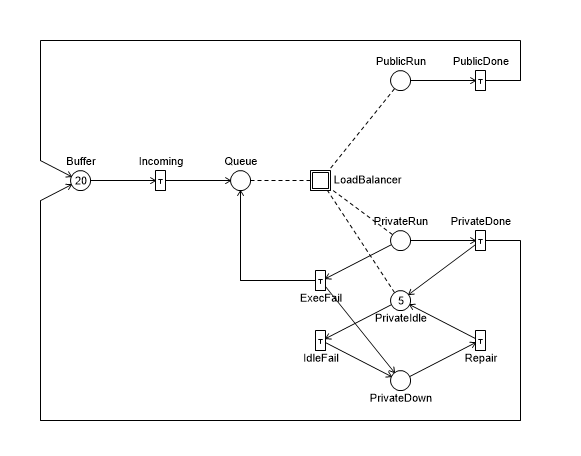
\includegraphics[width=140mm, keepaspectratio]{figures/hybc.png}
	\caption{Hibrid felhő modell a PetriDotNet alkalmazásban}
\end{figure}

\subsection{Philosophers}

A klasszikus "étkező filozófusok problémája", stochasztikus rendszerként modellezve.
Adva van valahány filozófus (esetünkben 3, 5, 7 illetve 9), akik egy kerek asztal körül ülnek. Mindegyikük előtt van egy tányér, a tányérok között félúton pedig egy-egy villa. Mindegyik filozófus elmélkedik, egészen addig, míg meg nem éhezik. Akkor azonban csak akkor tud étkezni, ha mindkét oldalán szabad a villa, ha valamelyik nem áll a rendelkezésére, várakoznia kell.

Modelleink esetében a paraméterek jelölik, milyen gyakran éheznek meg az egyes filozófusok, reward függvényeink pedig azt, hogy mennyit tudnak elmélkedni az este folyamán.
\begin{center}
	\begin{tabular}{cc}
		\textbf{\textbf{Paraméter}} & \textbf{Default érték} \\
		\hline
		phil1\_eatingRate & 7.33569408796258\\
		phil2\_eatingRate & 2.15637692896620\\
		phil3\_eatingRate & 9.68078350329879\\
		phil4\_eatingRate & 9.64067749052976\\
		phil5\_eatingRate & 9.47722968486562\\
		phil6\_eatingRate & 4.03202598762859\\
		phil7\_eatingRate & 3.01116461683996\\
		phil8\_eatingRate & 1.24807417152331\\
		phil9\_eatingRate & 6.63293781606486\\
	\end{tabular}
	\label{table:filparam}
	\quad
	\begin{tabular}{c}
		\textbf{\textbf{Reward függvény}}\\
		\hline
		phil1\_thinkingTime\\
		phil2\_thinkingTime\\
		phil3\_thinkingTime\\
		phil4\_thinkingTime\\
		phil5\_thinkingTime\\
		phil6\_thinkingTime\\
		phil7\_thinkingTime\\
		phil8\_thinkingTime\\
		phil9\_thinkingTime\\
	\end{tabular}
	\label{table:filrewards}
\end{center}

\begin{figure}
	\centering
	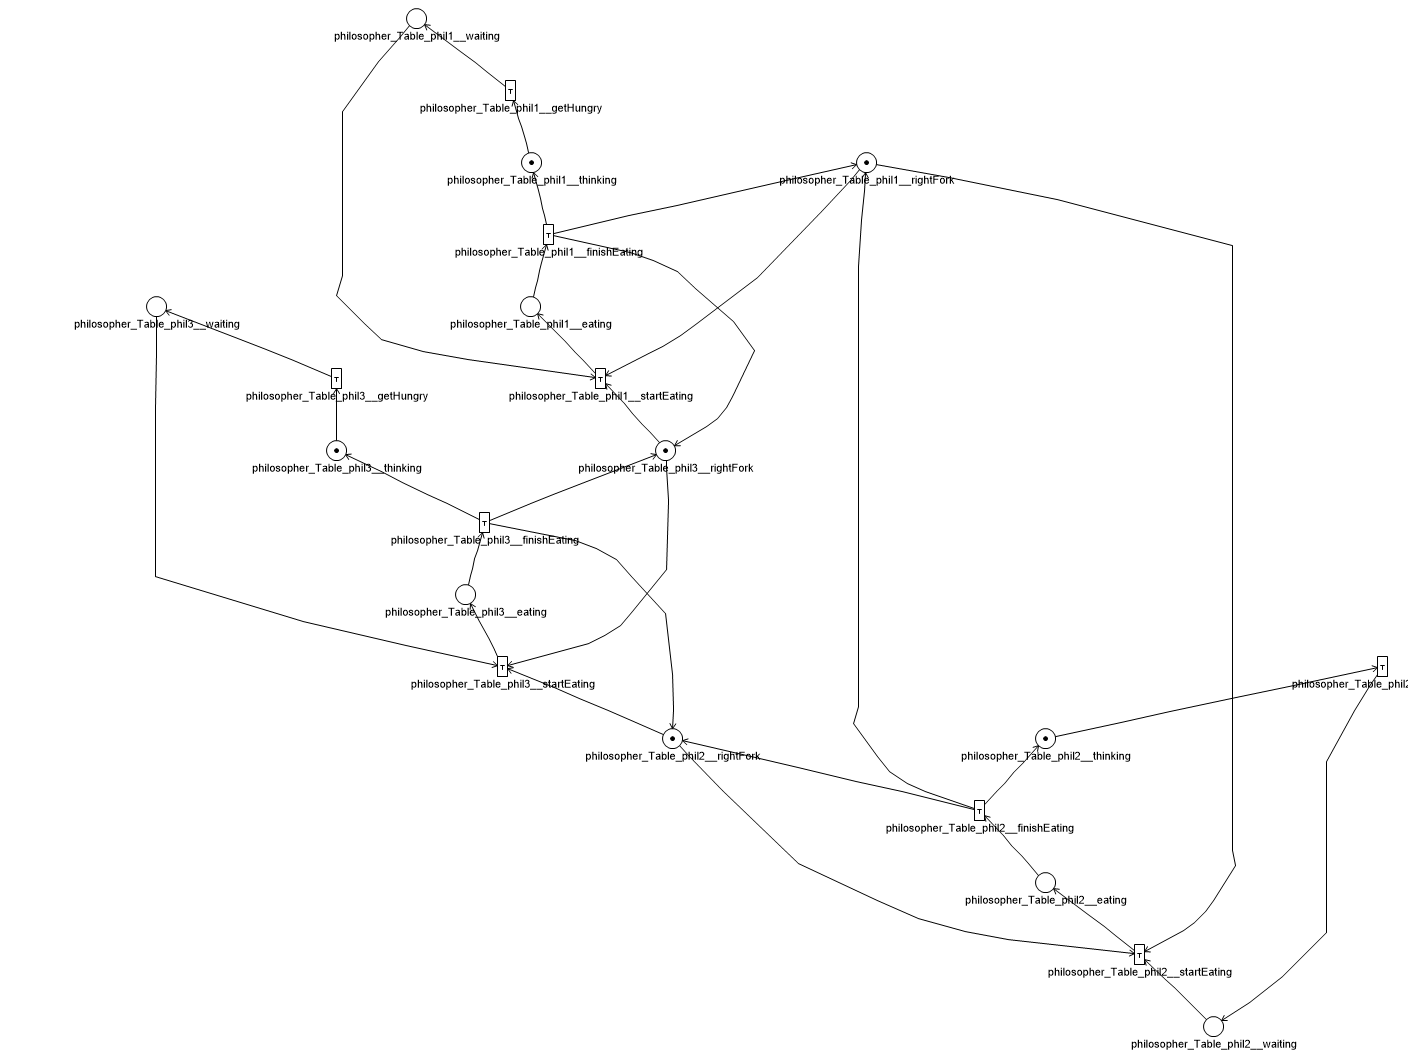
\includegraphics[width=150mm, keepaspectratio]{figures/fil3.png}
	\caption{3 filozófust tartalmazó modell a PetriDotNet alkalmazásban}
\end{figure}

%\label{page:last}
\end{document}
